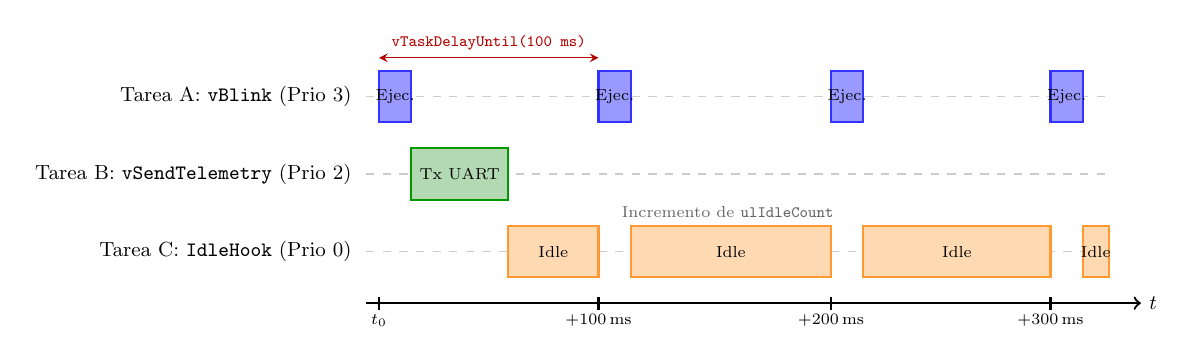
\begin{tikzpicture}[scale=0.82, transform shape, every node/.style={font=\small}]
  % Ejes de tareas
  \draw[->, thick] (0,0) -- (12,0) node[right] {$t$};
  \node[left] at (-0.1, 3.2) {Tarea A: \texttt{vBlink} (Prio 3)};
  \node[left] at (-0.1, 2.0) {Tarea B: \texttt{vSendTelemetry} (Prio 2)};
  \node[left] at (-0.1, 0.8) {Tarea C: \texttt{IdleHook} (Prio 0)};

  % Líneas base
  \draw[gray!40, dashed] (0, 3.2) -- (11.5, 3.2);
  \draw[gray!40, dashed] (0, 2.0) -- (11.5, 2.0);
  \draw[gray!40, dashed] (0, 0.8) -- (11.5, 0.8);

  % Tarea A (vBlink) - se ejecuta periódicamente cada 100 ms (pulsos breves)
  \fill[blue!40, draw=blue!80, thick] (0.2, 2.8) rectangle (0.7, 3.6) node[pos=0.5, black, font=\scriptsize] {Ejec.};
  \fill[blue!40, draw=blue!80, thick] (3.6, 2.8) rectangle (4.1, 3.6) node[pos=0.5, black, font=\scriptsize] {Ejec.};
  \fill[blue!40, draw=blue!80, thick] (7.2, 2.8) rectangle (7.7, 3.6) node[pos=0.5, black, font=\scriptsize] {Ejec.};
  \fill[blue!40, draw=blue!80, thick] (10.6, 2.8) rectangle (11.1, 3.6) node[pos=0.5, black, font=\scriptsize] {Ejec.};

  % Tarea B (vSendTelemetry) - ejecuta al inicio o cada 2 s, es desalojada o corre tras Tarea A
  \fill[green!50!black!30, draw=green!60!black, thick] (0.7, 1.6) rectangle (2.2, 2.4) 
    node[pos=0.5, black, font=\scriptsize] {Tx UART};

  % Tarea C (Idle Hook) - corre en todo el tiempo restante
  \fill[orange!30, draw=orange!80, thick] (2.2, 0.4) rectangle (3.6, 1.2) node[pos=0.5, black, font=\scriptsize] {Idle};
  \fill[orange!30, draw=orange!80, thick] (4.1, 0.4) rectangle (7.2, 1.2) node[pos=0.5, black, font=\scriptsize] {Idle};
  \fill[orange!30, draw=orange!80, thick] (7.7, 0.4) rectangle (10.6, 1.2) node[pos=0.5, black, font=\scriptsize] {Idle};
  \fill[orange!30, draw=orange!80, thick] (11.1, 0.4) rectangle (11.5, 1.2) node[pos=0.5, black, font=\scriptsize] {Idle};

  % Marcadores temporales
  \draw[thick] (0.2, -0.1) -- (0.2, 0.1) node[below=4pt, font=\scriptsize] {$t_0$};
  \draw[thick] (3.6, -0.1) -- (3.6, 0.1) node[below=4pt, font=\scriptsize] {$+100\,\mathrm{ms}$};
  \draw[thick] (7.2, -0.1) -- (7.2, 0.1) node[below=4pt, font=\scriptsize] {$+200\,\mathrm{ms}$};
  \draw[thick] (10.6, -0.1) -- (10.6, 0.1) node[below=4pt, font=\scriptsize] {$+300\,\mathrm{ms}$};

  % Flechas y anotaciones
  \draw[<->, >=stealth, red!70!black] (0.2, 3.8) -- (3.6, 3.8) 
    node[midway, above, font=\scriptsize] {\texttt{vTaskDelayUntil(100 ms)}};
  \node[above, font=\scriptsize, gray!80!black] at (5.6, 1.2) {Incremento de \texttt{ulIdleCount}};
\end{tikzpicture}
